\documentclass[12pt,a4paper]{article}
\usepackage[utf8]{inputenc}
\usepackage[T1]{fontenc}
\usepackage{amsmath}
\usepackage{textcomp}

\usepackage{geometry}
\geometry{a4paper,left=25mm,right=25mm, top=2cm, bottom=2cm} 

\usepackage{graphicx} %fuer bilder

\usepackage{verbatim}




 \usepackage{mathptmx}
 \usepackage[scaled=.90]{helvet}
 \usepackage{courier}



\usepackage{listings}
\usepackage{color}
 
\definecolor{dkgreen}{rgb}{0,0.6,0}
\definecolor{gray}{rgb}{0.5,0.5,0.5}
\definecolor{mauve}{rgb}{0.58,0,0.82}

\pagestyle{empty}
\lstset{numbers=left,language=C++}
\lstset{showstringspaces=false,
basicstyle=\ttfamily\footnotesize,
breaklines=true,
tabsize=3,
commentstyle=\color{dkgreen},      % comment style
inputencoding={ansinew},
title=\lstname %zeigt titel der datei an
}

\usepackage{pdfpages}% fuer pdfs



%keine einrückungen bei absatz
\parindent 0pt

\begin{document}
\title{Übung 01}
\author{Reinhard Penn, Bernhard Selymes}
\date{März 2015}

\normalsize

%Pfad zu c++ Dateien


%Beginn des Dokuments

\newcommand{\Uebung}{BFMVHDL}
\newcommand{\srcpath}{../../src}
\newcommand{\simpath}{../../sim}

%Angabe
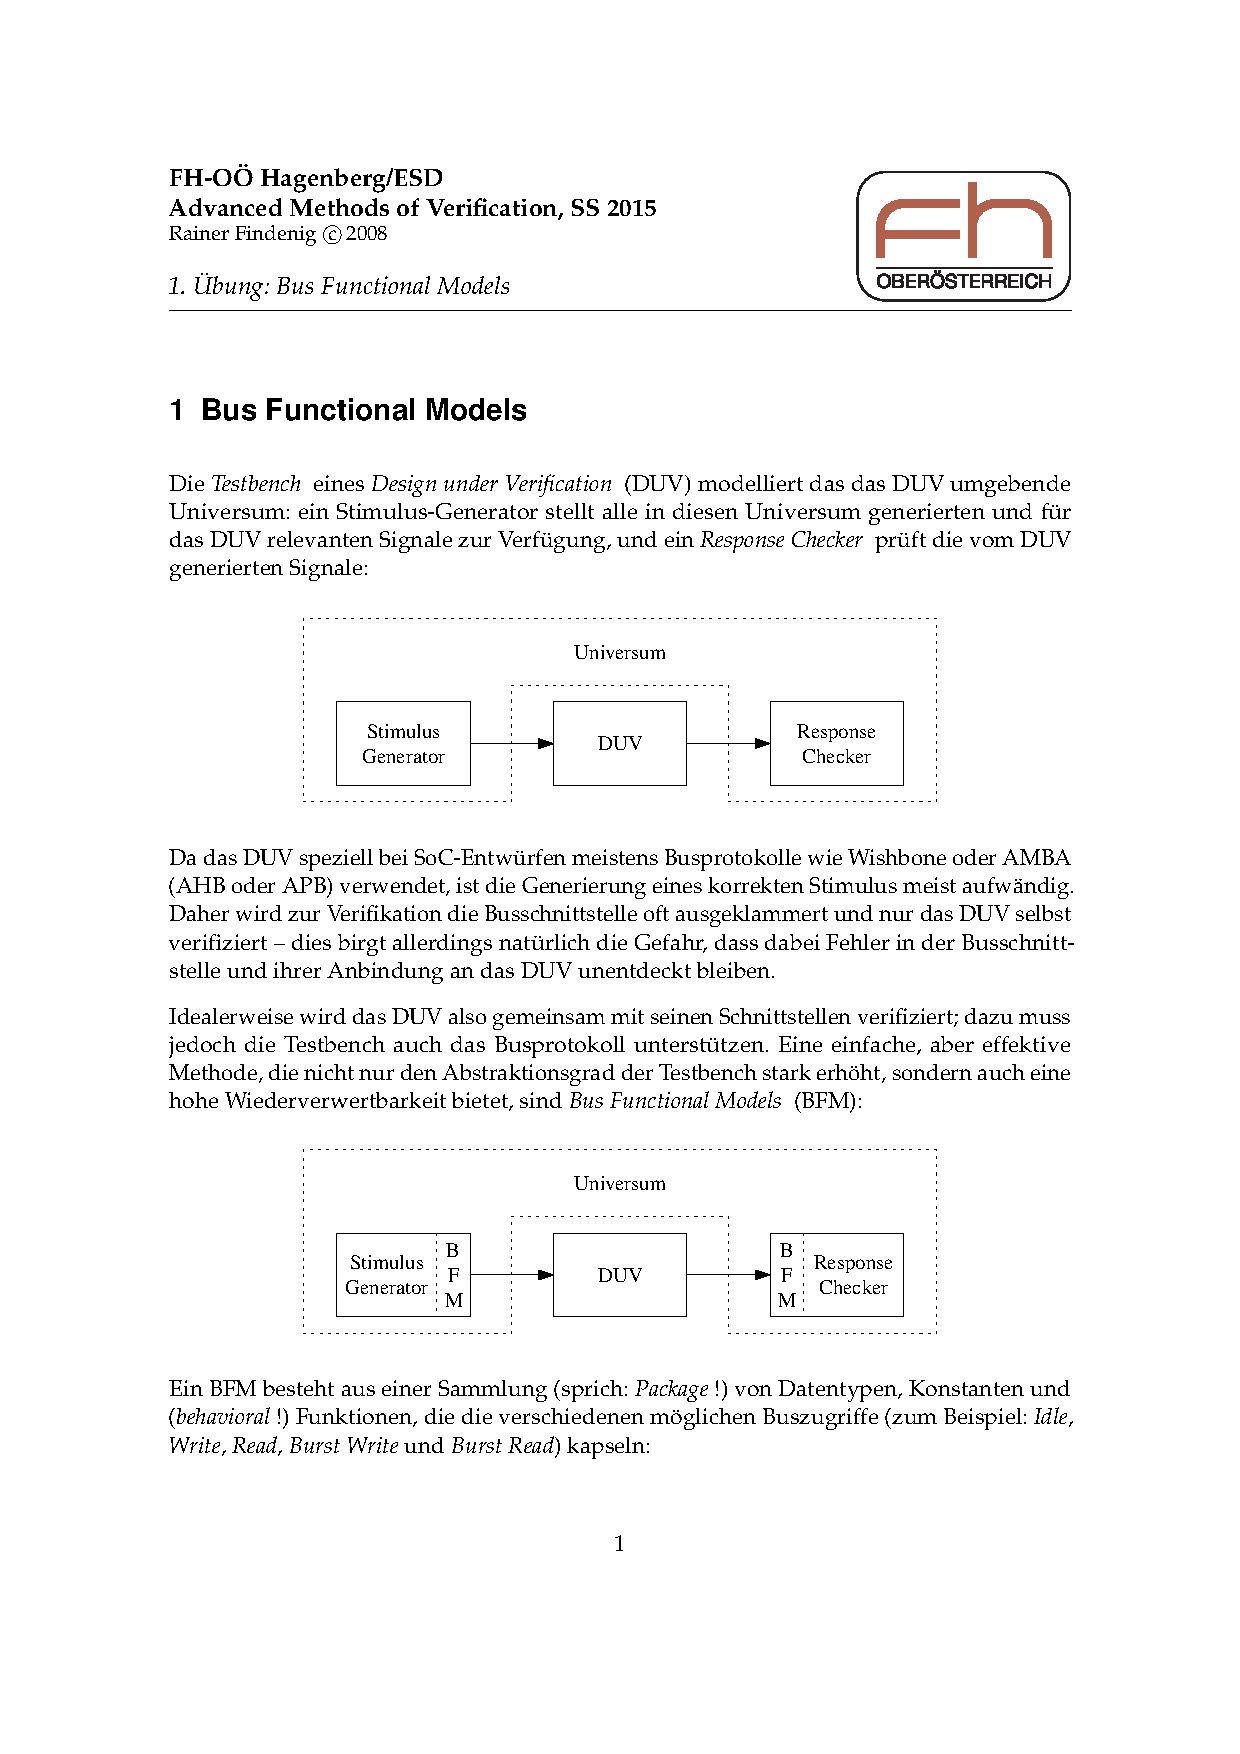
\includepdf[pages=-]{../Angabe.pdf}

\section{Beantwortung der Fragen}

\section{Source Code}

\lstinputlisting[language={VHDL}]{\srcpath/WishboneBFM-p.vhd}
\lstinputlisting[language={VHDL}]{\srcpath/WishboneBFM-tb.vhd}

\lstinputlisting[language={tcl}]{\simpath/Compile.do}
\lstinputlisting[language={tcl}]{\simpath/Sim.do}

\end{document}
